%%%%%%%%%%%%%%%%%%%%%%%%%%%%%%%%%%%%%%%%%%%%%%%%%%%%%%%%%%%%%%%%%%%%%%%%%%%%%%%%%%%%
% Do not alter this block (unless you're familiar with LaTeX
\documentclass{article}
\usepackage[margin=1in]{geometry} 
\usepackage{amsmath, amsthm, amssymb,amsfonts, fancyhdr, color, comment, graphicx, environ}
\usepackage{xcolor}
\usepackage{mdframed}
\usepackage[shortlabels]{enumitem}
\usepackage{indentfirst}
\usepackage{hyperref}
\usepackage{algorithm2e}
\usepackage{graphicx}
\usepackage{wrapfig}
\usepackage{hyperref}
\usepackage{listings}
\lstset{ 
  language=R,                     % the language of the code
  basicstyle=\normalsize\ttfamily, % the size of the fonts that are used for the code
  numbers=left,                   % where to put the line-numbers
  numberstyle=\normalsize\color{gray},  % the style that is used for the line-numbers
  stepnumber=1,                   % the step between two line-numbers. If it is 1, each line
                                  % will be numbered
  numbersep=5pt,                  % how far the line-numbers are from the code
  backgroundcolor=\color{white},  % choose the background color. You must add \usepackage{color}
  showspaces=false,               % show spaces adding particular underscores
  showstringspaces=false,         % underline spaces within strings
  showtabs=false,                 % show tabs within strings adding particular underscores
  frame=single,                   % adds a frame around the code
  rulecolor=\color{black},        % if not set, the frame-color may be changed on line-breaks within not-black text (e.g. commens (green here))
  tabsize=2,                      % sets default tabsize to 2 spaces
  captionpos=b,                   % sets the caption-position to bottom
  breaklines=true,                % sets automatic line breaking
  breakatwhitespace=false,        % sets if automatic breaks should only happen at whitespace
  keywordstyle=\color{black},      % keyword style
  commentstyle=\color{gray},   % comment style
  stringstyle=\color{teal}      % string literal style
} 
\hypersetup{
    colorlinks=true,
    linkcolor=blue,
    filecolor=magenta,      
    urlcolor=blue,
}


\pagestyle{fancy}


\newenvironment{problem}[2][Problem]
    { \begin{mdframed}[backgroundcolor=gray!20] \textbf{#1 #2} \\}
    {  \end{mdframed}}

% Define solution environment
\newenvironment{solution}
    {\textit{Solution:}}
    {}

\renewcommand{\qed}{\quad\qedsymbol}

% prevent line break in inline mode
\binoppenalty=\maxdimen
\relpenalty=\maxdimen

%%%%%%%%%%%%%%%%%%%%%%%%%%%%%%%%%%%%%%%%%%%%%
%Fill in the appropriate information below
\lhead{Pengju Zhang}
\rhead{CSC-424} 
\chead{\textbf{Assignment 4}}
%%%%%%%%%%%%%%%%%%%%%%%%%%%%%%%%%%%%%%%%%%%%%

\begin{document}
%problem 1
\begin{problem}{1}
\textbf{[20 pts]}
An academic paper from a conference or Journal will be posted to the Homework 2 content section of D2L. It contains a usage of Correspondence Analysis. Review the paper and evaluate their usage of the technique. In particular, address in detail the following points. You should be able to fill at least a page with your review and analysis, and each point should be answered in a complete paragraph with several sentences. If you claim something about the paper, you should be able to back it up with a quote or evidence from the paper.
\end{problem}
\begin{solution}
\begin{enumerate}
	\item Because of the requirement to see what traits connect to the perspectives individuals have about the various institutions, the data used in this study lends itself well to correspondence analysis. Correspondence analysis excels at handling the categorical character of response data. Researchers will be able to infer what patients/users think or associate with different hospitals if they can group corresponding opinions and factors with different hospitals. According to the authors of the research, correspondence analysis is excellent for dealing with the multidimensional character of the perceptual mapping problem as well as the complexity of the data presented in the graphical output.
	\item The study employs correspondence analysis to determine how different variables are linked to various hospitals. The study enlisted the help of a random sample of people from each of the hospitals' surrounding communities, who were asked to choose from a list of 13 attributes that they identified with the hospitals. To better understand patients' perceptions of hospitals, they employ category level variables such as expert emergency treatment (emer), cancer therapy (canc), and advanced technological equipment.
	\item They employ a two-dimensional graph based on two principal components produced via correspondence analysis for their analysis. The graph depicts both the features and the hospitals in a single figure. This is helpful for comprehending the underlying structure and placement of various features in relation to connected hospitals. They can utilize proximity as a barometer of the features that patients perceive different hospitals to have.
	\item While the study goes into detail on the amount of variance captured by the various components and why they believe that amount is appropriate, it does not evaluate the model's overall fit to the data. While some believe that the overall higher level of variance captured is a useful predictor of model fit, this alone is not sufficient to show overall model fit.
	\item The study does an excellent job of giving not only interpretability of the data but also practical lessons for both management and marketers. The Cleveland Clinic, for example, is most strongly associated with "cancer therapy, heart disease prevention, and having modern technological equipment," according to the report. This draws attention to the hospital's strengths while also allowing management to improve on specific areas of focus. Another intriguing interpretation of the findings is that clusters of hospitals located close together have little in common, suggesting methods for hospitals to differentiate themselves from their competition.
	\item Failure to assess the statistical significance of the dependence on the row variables vs the columns is one such omission. A chi-square test may have been used to do this. This would show that their findings were not influenced by the sample size and give the study more overall validity. This is significant since it demonstrates that the findings are not only valid but also reproducible.
\end{enumerate}
\end{solution}

\newpage
%problem 2
\begin{problem}{2}
\textbf{[20 pts]}
The file “Survey.csv” contains survey responses to a questionnaire about Wikepedia pages. Each question’s responses are on a 5 point likert scale. Perform an ordinal Principal Factor Analysis (exploratory) on this data addressing the following points. The questions are
\begin{enumerate}
	\item Compute the correlation matrix in three ways, first with the pearson correlation, second with the spearman rank correlation, third with the Kendall tau correlation, and visualize all three with the corrplot function. How do the correlation matrices differ.
	\item Compute the KMO test for sample adequacy and interpret it.
	\item Use the Spearman correlation matrix to conduct a first PCA for the data to choose a
number of factors to extract in your factor analysis. Explain your reasoning for your choice
of number.
	\item Use the Spearman correlation with the “principal” function from the psych package to
compute a principal factor analysis on the data using the number of components that you
found.
	\item Print the loadings with a proper cutoff and then attempt to interpret the results. Give a
name to each of the factors that describes what it encapsulates. Note any surprising connections between the variables in their contributions. In particular, are there any variable groupings that are different than the label groupings for the question above
	\item Evaluate the goodness of fit with the Chi-square and the RMSEA.
	\item Repeat the analysis with the polychoric correlation. The pysch package
has a nice polychoric function you can use.
\end{enumerate}
\end{problem}
\begin{solution}
\href{run:./src/p2.r}{ (Problem 2 Source Code)}
\begin{enumerate}
	\item\mbox{}
	\begin{figure}[h]
		\centering
		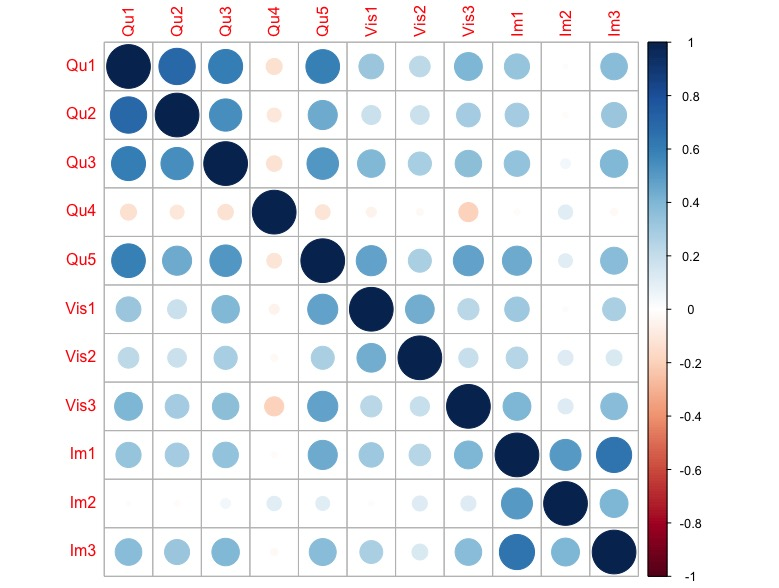
\includegraphics[width=0.5\textwidth]{Figure1_Pearson.jpeg}
		\caption{Pearson Scatter Plot}
	\end{figure}
	\begin{figure}[h]
		\centering
		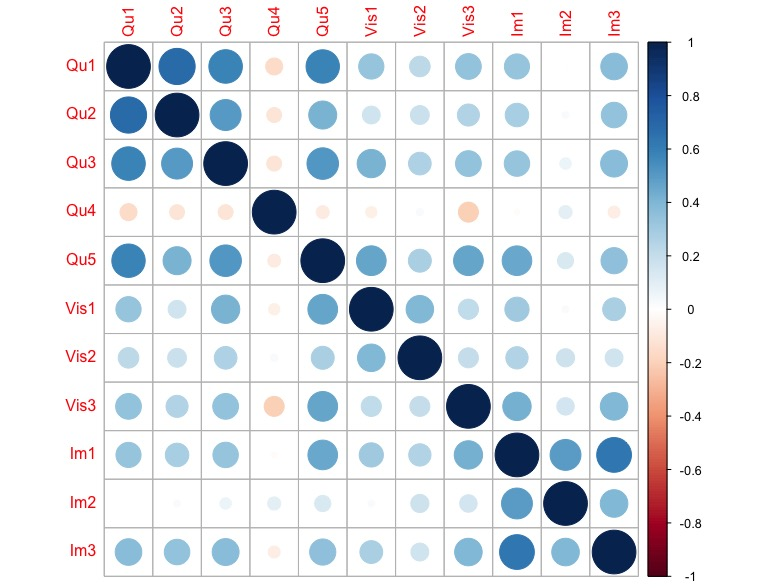
\includegraphics[width=0.5\textwidth]{Figure1_Spearman.jpeg}
		\caption{Spearman Scatter Plot}
	\end{figure}
	\begin{figure}[h]
		\centering
		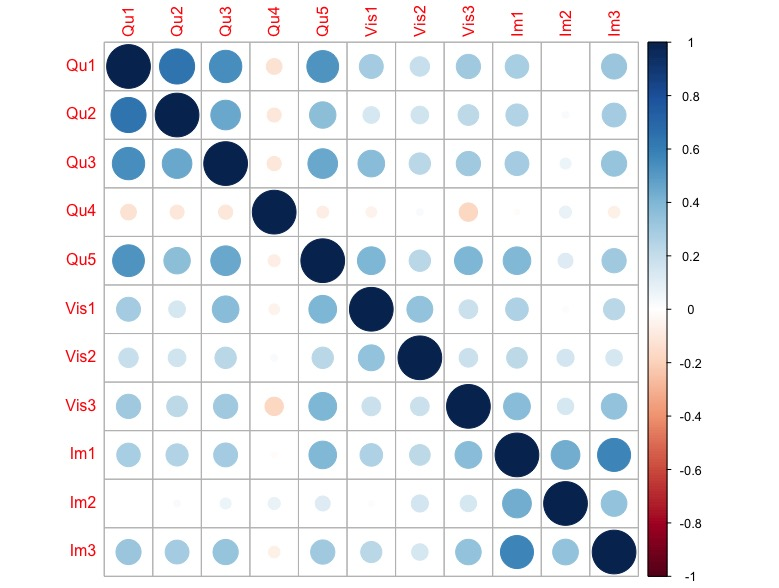
\includegraphics[width=0.5\textwidth]{Figure1_Kendall.jpeg}
		\caption{Kendall Scatter Plot}
	\end{figure}
\newpage
The variables vis2 and vis3 are swapped between Pearson and Spearman/Kendall, which is a major change. Because Spearman and Kendall correlation plots are created to produce correlations of ordinal data, but Pearson is supposed to be used on continuous data, we should consider them to be more accurate and insightful.
\item\mbox{}
	\begin{lstlisting}
> KMO(data)
# output
Kaiser-Meyer-Olkin factor adequacy
Call: KMO(r = data)
Overall MSA =  0.82
MSA for each item = 
 Qu1  Qu2  Qu3  Qu4  Qu5 Vis1 Vis2 Vis3  Im1  Im2  Im3 
0.82 0.79 0.91 0.75 0.88 0.76 0.77 0.89 0.79 0.65 0.83 
	\end{lstlisting}
We receive an MSA value of 0.82 when we run the Kaiser-Meyer Olkin test on our data. It is suggested that you aim for a number greater than 0.5/0.7. With a factor stability of 0.82, we can tell that we have enough sample depth to complete our study.
\item\mbox{}
	\begin{lstlisting}
> pca.spearman = prcomp(c2)
> summary(pca.spearman)
# output
Importance of components:
                          PC1    PC2    PC3     PC4     PC5     PC6     PC7     PC8     PC9    PC10      PC11
Standard deviation     0.6571 0.4339 0.3288 0.23042 0.22013 0.16332 0.15158 0.13413 0.10079 0.08371 1.701e-18
Proportion of Variance 0.4721 0.2059 0.1182 0.05805 0.05298 0.02917 0.02512 0.01967 0.01111 0.00766 0.000e+00
Cumulative Proportion  0.4721 0.6780 0.7962 0.85429 0.90727 0.93644 0.96156 0.98123 0.99234 1.00000 1.000e+00
	\end{lstlisting}
	\begin{figure}[h]
		\centering
		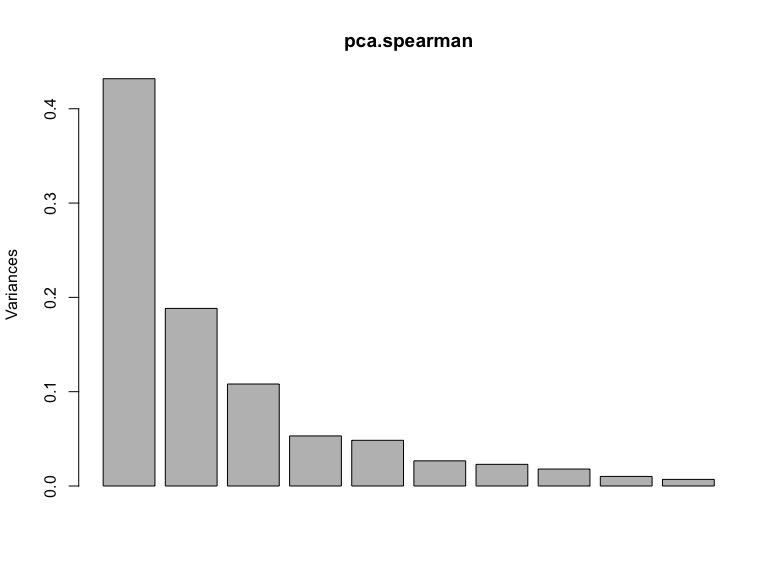
\includegraphics[width=0.7\textwidth]{Figure2_ScreePlot_Spearman.jpeg}
		\caption{Spearman Scree Plot}
	\end{figure}	
When we look at the principal components, we can see that three components account for 80\% of the variance. This could be an appropriate cutoff point, because we need to include two more components to gain an additional 10\% of captured variance.
According to the scree plot, there are three separate bars above the variance = 1 line, it still indicate the the first three components are decent cutoff point.
\newpage
\item\mbox{}
	\begin{lstlisting}
> pfa.spearman = principal(c2, nfactors = 3, rot = "none")
> pfa.spearman
# output
Principal Components Analysis
Call: principal(r = c2, nfactors = 3, rotate = "none")
Standardized loadings (pattern matrix) based upon correlation matrix
       PC1   PC2   PC3   h2   u2 com
Qu1   0.75 -0.40 -0.09 0.73 0.27 1.5
Qu2   0.64 -0.36 -0.19 0.58 0.42 1.8
Qu3   0.73 -0.27  0.07 0.62 0.38 1.3
Qu4  -0.17  0.33  0.51 0.40 0.60 2.0
Qu5   0.77 -0.12  0.09 0.61 0.39 1.1
Vis1  0.56 -0.11  0.53 0.61 0.39 2.1
Vis2  0.45  0.09  0.61 0.59 0.41 1.9
Vis3  0.61  0.07 -0.25 0.45 0.55 1.4
Im1   0.70  0.50 -0.10 0.76 0.24 1.9
Im2   0.31  0.79 -0.10 0.72 0.28 1.3
Im3   0.68  0.38 -0.25 0.67 0.33 1.9

                       PC1  PC2  PC3
SS loadings           4.09 1.53 1.12
Proportion Var        0.37 0.14 0.10
Cumulative Var        0.37 0.51 0.61
Proportion Explained  0.61 0.23 0.17
Cumulative Proportion 0.61 0.83 1.00

Mean item complexity =  1.6
Test of the hypothesis that 3 components are sufficient.

The root mean square of the residuals (RMSR) is  0.09 

Fit based upon off diagonal values = 0.93
	\end{lstlisting}
\newpage
\item\mbox{}
	\begin{lstlisting}
> print(pfa.spearman$loadings, cutoff = 0.4)
# output
Loadings:
     PC1    PC2    PC3   
Qu1   0.754              
Qu2   0.645              
Qu3   0.734              
Qu4                 0.512
Qu5   0.768              
Vis1  0.565         0.532
Vis2  0.450         0.614
Vis3  0.614              
Im1   0.702  0.503       
Im2          0.785       
Im3   0.680              

                 PC1   PC2   PC3
SS loadings    4.094 1.525 1.124
Proportion Var 0.372 0.139 0.102
Cumulative Var 0.372 0.511 0.613
	\end{lstlisting}
Component one, as seen in the factor loadings above, comprises substantial components from all variables except Qu4 and Im2. Qu4 has a small negative contribution, which is likely due to the fact that the question is reverse coded, which means that while a five would have been a positive feature on all of the other questions, the way the question is worded means that a high score, such as a 5, is actually a negative feature, which is the opposite of the other questions.
\item\mbox{}
	\begin{lstlisting}
> print(pfa.spearman) 
# output
Mean item complexity =  1.6
Test of the hypothesis that 3 components are sufficient.

The root mean square of the residuals (RMSR) is  0.09 

Fit based upon off diagonal values = 0.93
	\end{lstlisting}
\item\mbox{}
	\begin{lstlisting}
## Polychoric correlation
poly_cor = polychoric(data[1:11])
rho = poly_cor$rho
save(rho, file = "polychoric")
### Thresholds/Scaling results
poly_cor$tau
cor.plot(poly_cor$rho, numbers=T, upper=FALSE, main = "Polychoric Correlation", show.legend = FALSE)
load("polychoric")
# Scree plot
fa.parallel(rho, fm="pa", fa="fa", main = "Scree Plot")
	\end{lstlisting}
\end{enumerate}
\end{solution}

\newpage
%problem 3
\begin{problem}{3}
\textbf{[20 pts]}
Perform a correspondence analysis on the stores and ages data in StoresAndAges.csv. In this file you are provided with the table for the two sets of categories. In particular perform the following
\begin{enumerate}
	\item Create a mosaic plot of the two categorical variables.
	\item Plot the results of the correspondence analysis.
	\item With each store, create an age profile for the store. Which customer ages are most
highly and least highly represented. For each store, draw the scale for that store and demonstrate that age profile on the graph. What you are doing here is evaluating, for each store, the correspondence of each of the ages just like we did in class.
	\item What patterns can you discern form the plot? In particular look at the age category for each of the staff groups. Are there major differences in shopping patterns between the age groups? Review the class notes on how to read these plots.
	\item From the summary of the result, what percentage of the “inertia” do the first two eigenvectors account for? How many eigenvectors would we need to get to 80 of the inertia? How easy would it be to plot the data with this many dimensions?
\end{enumerate}
\end{problem}
\begin{solution}
\href{run:./src/p3.r}{ (Problem 3 Source Code)}
\begin{enumerate}
\item\mbox{}
	\begin{figure}[h]
		\centering
		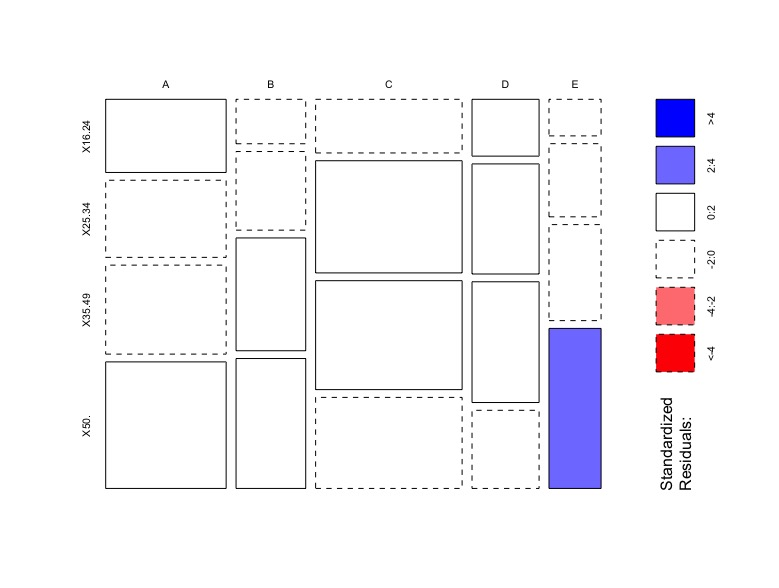
\includegraphics[width=0.7\textwidth]{Figrue3_MosaicPlot.jpeg}
		\caption{Mosaic Plot}
	\end{figure}
\newpage 
\item\mbox{}
	\begin{figure}[h]
		\centering
		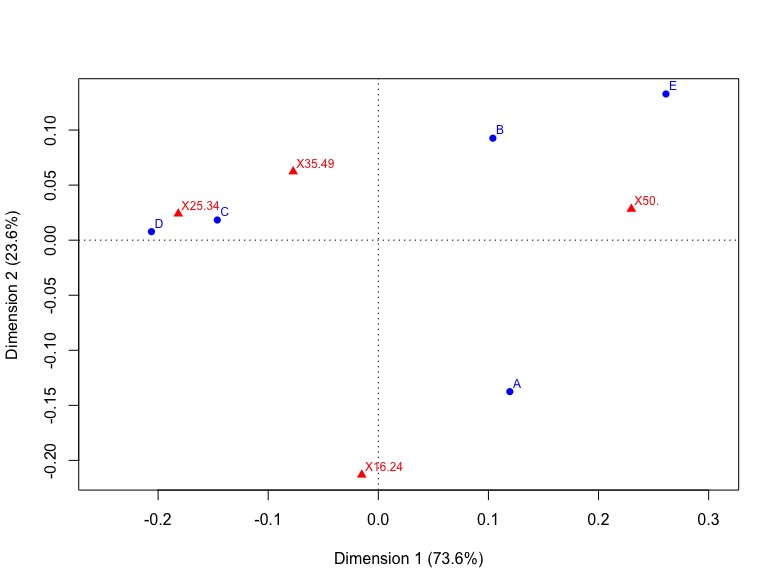
\includegraphics[width=0.7\textwidth]{Figure3_Correspondence.jpeg}
		\caption{Correspondence Plot}
	\end{figure}
\item
Store A: X16.24, X50.
\newline
Store B: X50, X35.49
\newline
Store C: X25.34, X35.49, X16.24
\newline
Store D: X25.34, X35.49, X16.24 
\newline
Store E: X.50, X35.49
\item
Stores B and E appear to have a substantially higher possibility of detecting elderly consumers, those over the age of 50. While the chart appears to imply that shops D and C have fewer elderly consumers and more customers in the range of 25-34 and 35-49 age groups.
\newpage
\item\mbox{}
	\begin{lstlisting}
> summary(c)
# output
Principal inertias (eigenvalues):

 dim    value      \%   cum\%   scree plot               
 1      0.026345  73.6  73.6  ******************       
 2      0.008443  23.6  97.2  ******                   
 3      0.001008   2.8 100.0  *                        
        -------- -----                                 
 Total: 0.035797 100.0                                 


Rows:
    name   mass  qlt  inr    k=1 cor ctr    k=2 cor ctr  
1 |    A |  264 1000  245 |  119 430 143 | -138 570 592 |
2 |    B |  153  889   93 |  104 496  63 |   93 393 155 |
3 |    C |  321  961  203 | -146 946 261 |   18  15  13 |
4 |    D |  147  966  181 | -206 965 237 |    8   1   1 |
5 |    E |  114  986  278 |  261 784 296 |  133 202 239 |

Columns:
    name   mass  qlt  inr    k=1 cor ctr    k=2 cor ctr  
1 | X162 |  153  997  196 |  -15   5   1 | -213 992 822 |
2 | X253 |  254  954  250 | -182 937 318 |   24  16  17 |
3 | X354 |  286  843   93 |  -77 512  65 |   62 332 131 |
4 |  X50 |  307  997  461 |  230 982 615 |   28  15  29 |
	\end{lstlisting}
Looking at the summary results from our correspondence analysis, we can see that we can capture 97.2 percent of the inertia using simply the first two eigenvectors. We'd like to include two eigenvectors to ensure that at least 80 percent of the inertia is caught, however it's worth noting that the first component captures 73.6 percent of the inertia. It would not be difficult to plot the data with only two dimensions because it would be simple to grasp and see, as well as simplify the data's overall interpretability.
\end{enumerate}
\end{solution}

\newpage
%problem 4
\begin{problem}{4}
\textbf{[20 pts]}
A common application of Discriminant Analysis is the classification of bonds into various bond rating classes. These ratings are intended to reflect the risk of the bond and influence the cost of borrowing for companies that issue bonds. Various financial ratios culled from annual reports are often used to help determine a company’s bond rating.
\begin{enumerate}
	\item What is the performance of the classifier on the training data? Notice that there is order in the class variables (i.e., AAA is better than AA, which is better than A,...).
	\item What is the performance of the classifier on the validation data?
	\item Would certain misclassification errors be worse than others? If so, how would you
suggest measuring this?
\end{enumerate}
\end{problem}
\begin{solution}
\href{run:./src/p4.r}{ (Problem 4 Source Code)}
\begin{enumerate}
\item\mbox{}
	\begin{figure}[h]
		\centering
		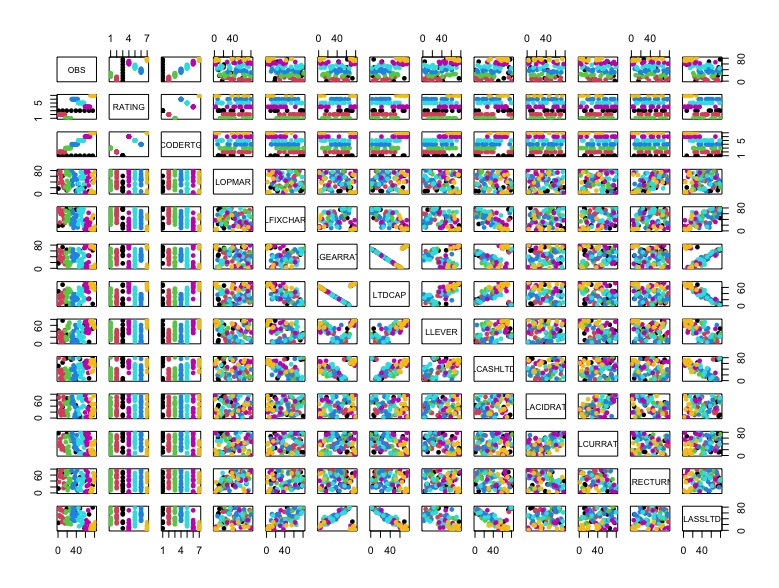
\includegraphics[width=0.7\textwidth]{Figure4_General.jpeg}
		\caption{Training Dataset Scatter Plot}
	\end{figure}
\newline
Generally we could not find much separation at the very beginning stage.
\newpage
	\begin{figure}[h]
		\centering
		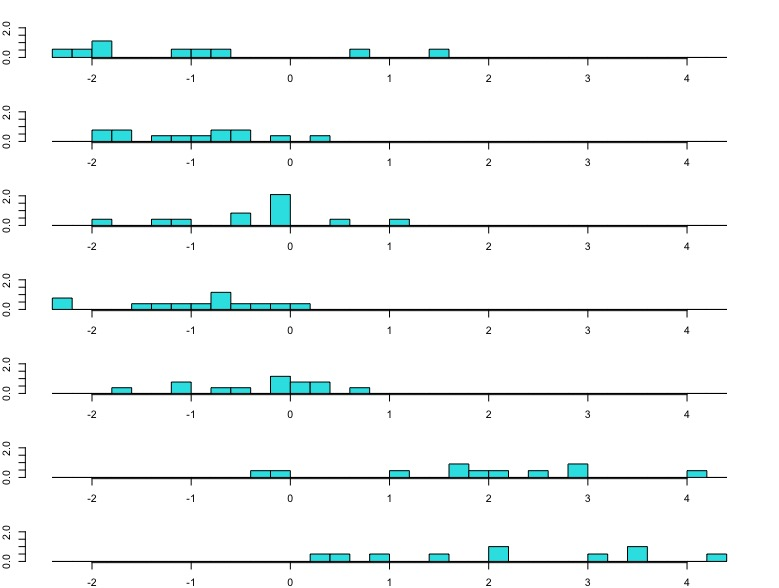
\includegraphics[width=0.6\textwidth]{Figure4_a_1.jpeg}
		\caption{Training Dataset Histogram Seperation}
		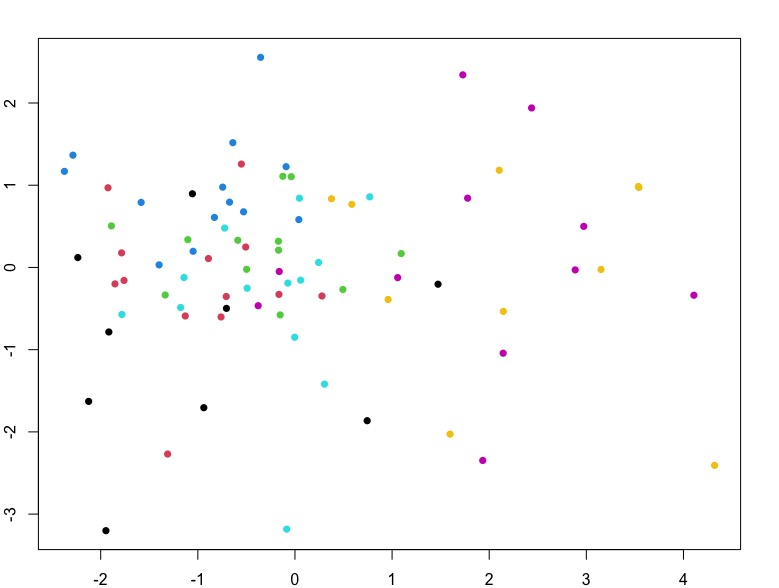
\includegraphics[width=0.6\textwidth]{Figure4_a_2.jpeg}
		\caption{Training Dataset Plot Seperation}
	\end{figure}
When we plot the histogram as shown below, we can see that there is a lot of overlap and poor group separation. We notice outliers high above 0 in group one, with the majority falling between -2 and -1. The plotting of the findings reveals no improvement, and the group separation still looks to be heavily overlapping. We can acquire some useful insight by looking at the confusion matrix with true values on the rows and anticipated values on the columns. The model's failure to reduce within-class dispersion while increasing out-of-class scatter demonstrates poor performance and gives few interpretable visual ques.
\newpage
\item\mbox{}
	\begin{figure}[h]
		\centering
		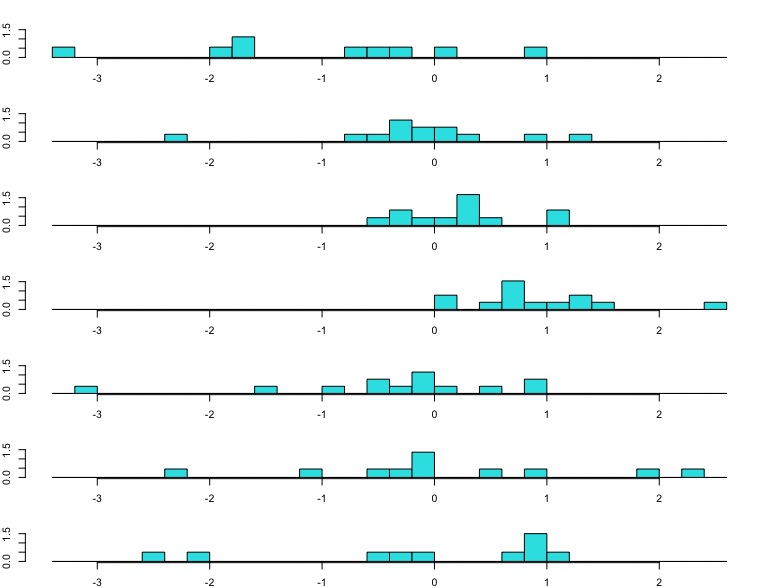
\includegraphics[width=0.6\textwidth]{Figure4_b_1.jpeg}
		\caption{Validation Dataset Histogram Seperation}
		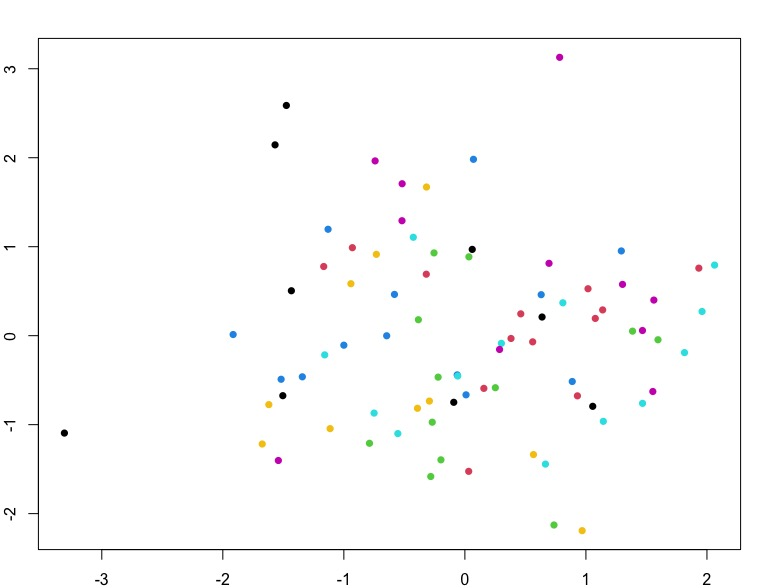
\includegraphics[width=0.6\textwidth]{Figure4_b_2.jpeg}
		\caption{Validation Dataset Plot Seperation}
	\end{figure}
\newpage
\item\mbox{}
	\begin{lstlisting}
> table(validationData$CODERTG, validationData.lda.predict$class)
  # output
    1 2 3 4 5 6 7
  1 1 0 0 1 0 0 0
  2 0 2 0 0 0 0 0
  3 0 0 1 1 0 0 0
  4 0 0 0 2 0 0 0
  5 0 1 0 1 0 0 0
  6 0 0 0 0 0 2 0
  7 0 0 0 0 0 0 2
	\end{lstlisting}
We can look at the many errors generated by our forecasts and determine which ones are more common than others. The worst of the various types of mistakes you may make appears to be designating a bond as not dangerous when it is actually exceedingly risky, as this would mean investments could be lost when the underlying asset was thought to be stable. This is in contrast to misclassifying a safe investment as dangerous and thus either avoiding the investment or accepting less risk than anticipated.
\end{enumerate}
\end{solution}
\end{document}